\chapter{Related Work}
\label{sec:Related Work}
This chapter introduces some foundational work on density-based and subspace/correlation clustering and gives an insight into existing approaches to solve the problem of subspace clustering. We also elaborate, where these existing approaches lack in ability and capability and show some of the current optimization approaches.

Since sections \nameref{sec:houghintro}, \nameref{sec:cashintro}, \nameref{sec:dbscanintro} and \nameref{sec:OPTICSintro} are essential to our work they will be elaborated in greater detail in the chapter \nameref{sec:Foundations}

\section{Hough Transformation}\label{sec:houghintro}
The Hough Transform originally was introduced by \textcite{houghOriginal1962method} and extended by \textcite{rosenfeld1969picture} in the field of computer vision for edge detection\cite{houghhistoryhart2009hough}. The initial purpose of the Hough transform was a technique to detect colinear points in an image space but has since then found various other applications in fields like image processing/analysis~\cite{rosenfeld1969picture,ballard1981generalizing}, computer vision~\cite{davies2004machine} and subspace clustering\cite{CASHachtert2008robust}.
The basic idea of the Hough transform is the transformation of all points $p_i = (x_i,y_i)$ in a 2-dimensional image space $\mathcal{D} \subseteq \R^2$ to functions $f_{p_i}$ in a 2-dimensional parameter space $\mathcal{P} \subseteq \R^2$, also known as Hough space\cite{illingworth1988survey}. This is can be done by e.g. taking a representation of a point $p$ as all of its concurrent lines $y_p = m \cdot x_p + t$ and rearranging it to $m_{p} = - \frac{1}{x_p} \cdot t_{p} + \frac{y_p}{x_p}$ which produces a straight with slope $m$ and y-intersect $t$ in a $(m,t)$-parameter space. Since each point in parameter space represents a particular $(m,t)$-setting, multiple functions close to each other implies that their respective points have similar $(m,t)$-settings as well. The correlation clustering objective therefore transforms to a density-based clustering objective in parameter space, with the added benefit of being able to detect correlating points regardless of their distance to each other in data space. This property is exploited by e.g. evaluating the whole parameter space in a grid or by smartly splitting the parameter space in \autoref{sec:houghintro} to detect linear correlations. 
\todor{Ich plagiere mich selbst. 1zu1 aus unterem abschnitt}
\begin{figure}
    \centering
    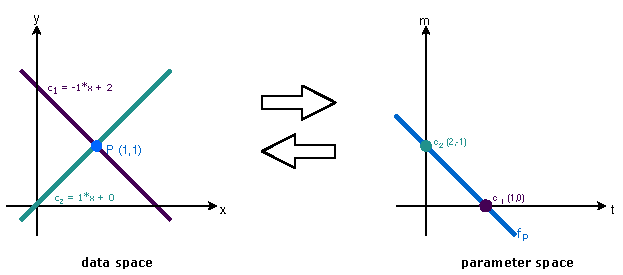
\includegraphics{figures/HoughMXT.pdf}
    \caption{Caption}
    \label{fig:houghmxt}
\end{figure}\todor{eher keine bilder in related work}

\section{CASH}\label{sec:cashintro}
\ac{CASH} extends the use case of the Hough Transformation to the detection of arbitrary-dimensional data spaces by augmenting the initial rigid 2-dimensional definition to a multi-dimensional one. Furthermore \ac{CASH} introduces a improved search strategy for detecting regions of high intersections in parameter space to improve the efficiency compared to the basic grid search \cite{CASHachtert2008robust}. Instead of doing an extensive count operation/accumulation of over a fixed interval, \ac{CASH} successively splits the whole parameter space by its axes and only evaluates hyperspace Since our work focuses on ``Detecting Global Correlated Clusters using Hough Transform through Locally Dense Correlations'', we use \ac{CASH} to cope with multi-dimensional data.\\

A more profound explanation to the transformation and its usage in \ac{CASH} will be given in \autoref{ssec:houghindepth}.


\section{DBSCAN}\label{sec:dbscanintro}
\citeauthor{DBSCANEKSX96} created a foundational algorithm with \ac{DBSCAN}. With over sixteenthousand citations on google scholar as of December 2019 it is one of the most influential works created in the field of density-based clustering. 

\section{OPTICS}\label{sec:OPTICSintro}
\cite{opticsankerst1999optics}
% Maybe OPTICS? DIRECTLY COPIED OUT OF \cite{ankerst1999optics}
%  First, almost all clustering algorithms require values for input parameters which are hard to
% determine, especially for real-world data sets containing highdimensional objects. Second, the algorithms are very sensible to
% these parameter values, often producing very different partitionings of the data set even for slightly different parameter settings.
% Third, high-dimensional real-data sets often have a very skewed
% distribution that cannot be revealed by a clustering algorithm using only one global parameter setting. 

\section{Current Optimization Approaches}
    (D-MASC\cite{kazempour2018d, kazempour2019galaxy}, A Galaxy of Correlations etc.) [0.5]
    
\section{Other Subspace Clustering Algorithms}
There are many other approaches to find relevant subspaces/correlations in data. Like \ac{ORCLUS} and \ac{4C}, many of them are based on the application of the \ac{PCA} to extract the correlations. This subsection introduces some of those subspace algorithms and explains, in which way those works would or would not be suited for our idea.

\subsection{ORCLUS}

\subsection{4C and COPAC}

\subsection{HiCO and ERiC}
(Global) Correlation Clustering, other algorithms so far (ORCLUS \cite{orclusaggarwal2000finding}, LMCLUS \cite{}, 4C, HiCO, ERiC)[1]